
%(BEGIN_QUESTION)
% Copyright 2007, Tony R. Kuphaldt, released under the Creative Commons Attribution License (v 1.0)
% This means you may do almost anything with this work of mine, so long as you give me proper credit

This electronic circuit requires only a single opamp to implement full PID control, given an error signal input.  Its characteristic equation is called {\it series} or {\it interacting}:

$$\includegraphics[width=15.5cm]{i01847x01.eps}$$

$$m = K_p \left[ \left({\tau_d \over \tau_i} + 1 \right) e + {1 \over \tau_i} \int e \> dt + \tau_d {de \over dt} \right] + b $$

\vskip 10pt

Identify which variable resistors influence the aggressiveness of the P, I, and D control actions in this mechanism.  

\begin{itemize}
\item{} Valve(s) influencing the controller's proportional action:
\vskip 10pt
\item{} Valve(s) influencing the controller's integral action:
\vskip 10pt
\item{} Valve(s) influencing the controller's derivative action:
\vskip 10pt
\item{} Which direction to move the potentiometer wiper for a {\it greater} proportional band: ({\it up} or {\it down})
\end{itemize}

\underbar{file i01847}
%(END_QUESTION)





%(BEGIN_ANSWER)

I recommend 2 points for each correct resistor answer, plus 4 points for the proper wiper movement:

\vskip 10pt

Variable resistor(s) influencing the controller's proportional action: ${\bf R_1}$, ${\bf R_2}$, and ${\bf R_{pot}}$

\vskip 10pt

Variable resistor(s) influencing the controller's integral action: ${\bf R_1}$ (okay if student mentions ${\bf R_{pot}}$ as well)

\vskip 10pt

Variable resistor(s) influencing the controller's derivative action: ${\bf R_2}$ (okay if student mentions ${\bf R_{pot}}$ as well)

\vskip 10pt

Which direction to move the potentiometer wiper for a {\it greater} proportional band: {\bf up}


%(END_ANSWER)





%(BEGIN_NOTES)

{\bf This question is intended for exams only and not worksheets!}.

%(END_NOTES)


